\documentclass[a4paper,9pt]{article}

\usepackage{anysize}
\usepackage{fancyhdr}
\usepackage{soul}
\usepackage[dvipsnames]{xcolor}
\usepackage{hyperref}
\usepackage{lipsum}
\usepackage{amsmath}
\usepackage{amssymb}
\usepackage{graphicx}
\usepackage{multicol}
\usepackage{parskip}
\usepackage{float}
\usepackage[backend=biber]{biblatex}
\usepackage[font=scriptsize]{caption}

% settings
\addbibresource{test/references.bib}

\marginsize{2cm}{2cm}{1cm}{2cm}
\renewcommand{\headrulewidth}{0pt}

\hypersetup{
    colorlinks=true,
    linkcolor=black,
    citecolor=CadetBlue,
    filecolor=CadetBlue,      
    urlcolor=CadetBlue,
}
  
\setlength\columnsep{18pt}
\renewenvironment{abstract}
 {\par\noindent\textbf{\abstractname}\ \ignorespaces \\}
 {\par\noindent\medskip}
 
 
\begin{document}

% Header
\pagestyle{fancy}
\thispagestyle{empty}
\fancyhead[R]{\textit{University of Groningen}}
\fancyhead[L]{}

\renewcommand*{\thefootnote}{\fnsymbol{footnote}}

\begin{center}
\Large{\textbf{Gyroscope}}
\vspace{0.4cm}
\normalsize
\\ Artur Topal, Tyn Rendering \\
\vspace{0.1cm}
\textit{University of Groningen}
\medskip
\normalsize
\end{center}

{\color{gray}\hrule}
\vspace{0.4cm}

\begin{abstract}
\lipsum{1}

\end{abstract}

{\color{gray}\hrule}
\medskip

\section{Introduction}

\lipsum{120}

In a closed damped driven oscillatory system, three forces are acting on a point mass: restoring force ($F_{restoring} = -kx$), damping force ($F_{damping} = -b\dot{x}$), and driving force ($F_{driving} = F_0 \cos(\omega_d t)$). By the Second Newton's law, resulting motion is modelled by:
\begin{equation*}
    m\ddot{x} + b\dot{x} + kx = F_0 \cos(\omega_d t)
\end{equation*}

More commonly, this differential equation is written as
\begin{equation} \label{eq:full_motion}
    \ddot{x} + 2\gamma \dot{x} + \omega^2 x = \frac{F_0}{m} \cos(\omega_d t)
\end{equation} where $\gamma = \frac{b}{2m}$ is the damping factor, $\omega = \sqrt{\frac{k}{m}}$ is natural angular frequency of the oscillations.

% refer to Morin for further information
Depending on the value of $\Omega^2$, there are three cases to consider: \textbf{underdamping}, \textbf{overdamping}, and \textbf{critical damping}. In this experiment, the damping factor was chosen in a way that the oscillatory system is underdamped ($\Omega^2 < 0$). In this case, after long enough time, the inital oscillations will die out, and the system will oscillate with some amplitude $A$ at the driving frequency $\omega_d$ but shifted by some phase $\phi$.
The amplitude can be found to be:
\begin{equation} \label{eq:full_motion_ampl}
  A = \frac{ F_d/m  }{ \sqrt{ (\omega^2 - \omega_d^2)^2 + (2\gamma \omega_d)^2 } }
\end{equation}
The phase is:
\begin{equation} \label{eq:full_motion_phase}
  \tan(\phi) = \frac{2 \gamma \omega_d}{\omega^2 - \omega_d^2}
\end{equation}

There is one frequency when the amplitude from Eq.~\eqref{eq:full_motion_ampl} is maximized. This particular frequency is called \textbf{resonance frequency}, $\omega_{res}$. The behavior of the damped driven oscillatory system at resonance frequency is further addressed in appendix \ref{appendix:preps}.  

In this experiment, the system is modelled using above equations since the restoring force comes from the springs, driven force is harmonic, and the damping force depends on the change of magnetic flux, which in our case depends on the speed. The only difference is that displacements ($x(t)$) and speeds are angular.  

\section{Methods}

\subsection{Equipment and preparations}

1. A \textbf{power supply} capable of giving $1000V$ or $30V$ DC.

2. A \textbf{parallel plate capacitor} with adjustable separation between the plates.

3. An \textbf{electrometer} capable of detecting small currents and measuring voltage in ranges, among others, $100V$ and $30V$. The range is selected with the FUNCTION knob. Besides, it must be discharged set the gauge needle set to $0V$ using the PUSH TO ZERO and/or ZERO LOCK knobs. The electrometer is grounded by connecting its $GND$ wire to the $GND$ pin of the power supply.

4. For grounding, the \textbf{grounding wrist bracelet} is used. It is grounded by connecting the bracelet wire to the $GND$ pin of the power supply.

5. The \textbf{Faraday cage}. It must be grounded by touching the inner and outer cage simultaneously with a grounded object (e.g., a hand with the wrist bracelet), and then releasing the inner cage and thereafter the outer cage.

6. A \textbf{black disk-on-a-rod}. It is further referred to as the rod.

7. A \textbf{conducting sphere} used as a charging station for the rod. It gains its electric potential by connecting it to the $1000V$ pin of the power supply.

\subsection{The capacitor voltage as a function of charge}

The separation of the capacitor is set to $d_{1} = 2 (mm)$. The conducting sphere is charged\footnote{On each iteration, the conducting sphere must be charged again, so that on every touch by the rod it has 1000V, and the rod gains the same charge each time.} to $1000V$ and placed at a distant from the capacitive circuit place. And the capacitor is connected to the electrometer like shown in figure \ref{methods:fig:capacitor_voltage}. The rod is touched to the sphere to gain some charge, and then to the isolated (positive) plate of the capacitor to transfer this charge. The electrometer's measurement is noted. The table of the capacitor voltage as a function of the number of charges is made (12 measurements). Each measurement is sampled twice.  

\begin{figure}[H]
  \centering
  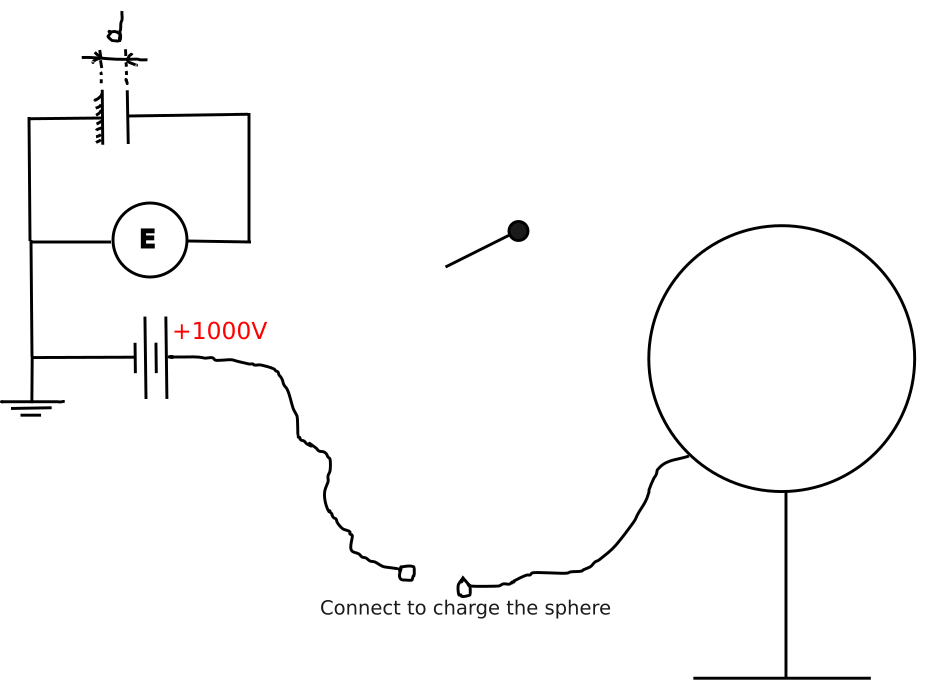
\includegraphics[width=0.5\textwidth]{capacitors/img/capacitor_voltage.png}
  \caption{The circuit for the finding the capacitor voltage as a function of charge}
  \label{methods:fig:capacitor_voltage}
\end{figure}

Then, the separation of the capacitor is set to $d_{2} = 4 (mm)$ and the same algorithm is conducted.

\subsection{The distribution of charge on a surface}

The capacitor is connected to the $1000V$ pin of the power supply like shown in figure \ref{methods:fig:distribution}. The electrometer is connected to the inner and outer cages of the Faraday cage. On each charge transfer, the Faraday cage and the rod are discharged. On each iteration, the rod is touched to the positive plate of the capacitor at some position, and the charge of its vicinity will be transferred to the rod. Then, the rod is put inside the Faraday cage, causing the capacitive voltage to appear between the inner and outer cage. This voltage is used as a measure of charge on the rod. This is iterated at different positions along the diameter of the capacitor plate (12 measurements). Each position is sampled twice.

\begin{figure}[H]
  \centering
  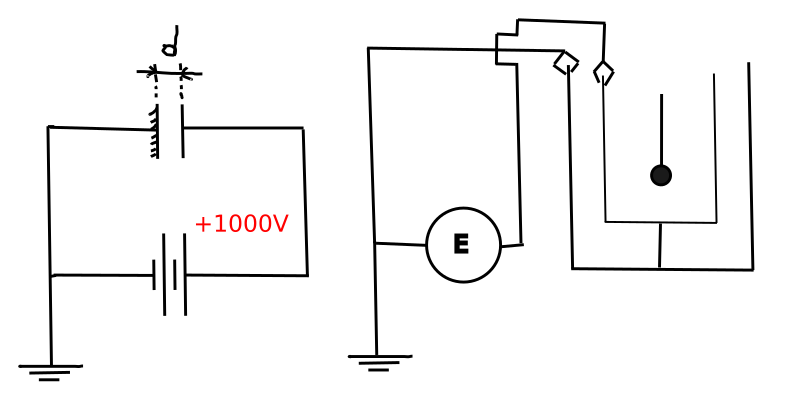
\includegraphics[width=0.5\textwidth]{capacitors/img/distribution.png}
  \caption{The circuit for the finding the surface charge distribution on the capacitor plate}
  \label{methods:fig:distribution}
\end{figure}

The \textit{surface charge density} is obtained from the voltage-position graph.

\subsection{The potential difference as function of the plate distance at constant charge}

The capacitor plate separation is initially set to $d_{1} = 2 (mm)$. The capacitor is charged with the $20V$ output from the power supply, and this charge remains stored in the capacitor after disconnecting the power supply. The electrometer's range is set to $-30V$ to $30V$. The capacitor voltage is measured for different capacitor plate separations from $d_{1} = 2 (mm)$ up to the maximum distance possible (in total 12 measurements). Each measurement is sampled twice.  

\subsection{Direct Calculation of Damping} \label{sec:direct_damping}

The oscillations produced without an added damping factor, i.e. the magnet are displayed in Figure 2. The assumption was made that the string to which the springs were attached did not slip from the pulley. Figure 2 shows underdamped oscillations, which can be seen by a decrease in amplitudes. The oscillations produced without an added damping factor, i.e. the magnet are displayed in \ref{fig:undamped_oscillations}. The assumption was made that the string to which the springs were attached did not slip from the pulley.

\begin{figure}[h!]
  \centering
  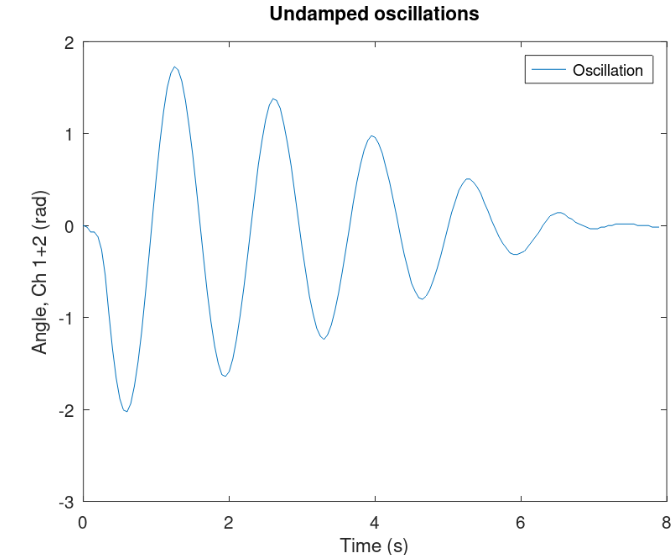
\includegraphics[width=1\textwidth]{oscillations/images/Undamped_Oscillations}
  \caption{Oscillations without damping}
  \label{fig:undamped_oscillations}
\end{figure}

From the measurements the coordinates of the maxima were determined and from this the natural frequency was determined to be $\omega = 4.8 \pm 0.1 (rad/s)$, which was constant throughout the measurements.

A damping term was added by placing the magnet back in its original position, the oscillations are displayed in \ref{fig:underdamped}. The coordinates of nine of the maxima were determined and were plotted in \ref{fig:log of damping factor}. 

\begin{figure}[h!]
  \centering
  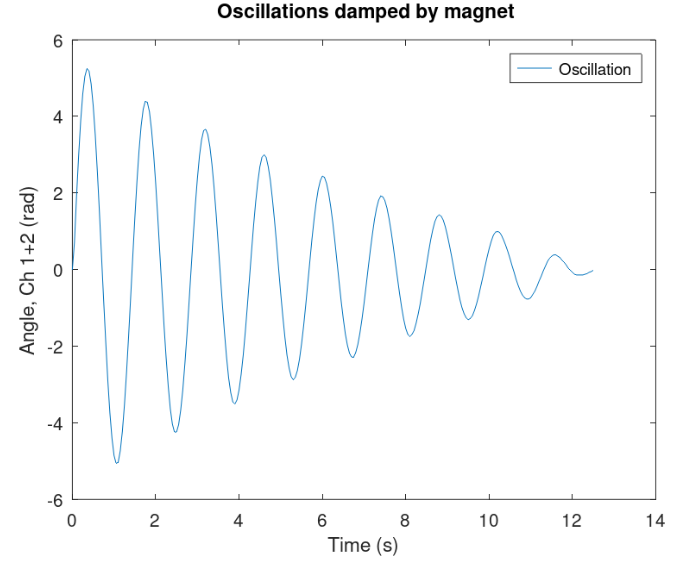
\includegraphics[width=1\textwidth]{oscillations/images/underdamped}
  \caption{Decrease in amplitude by an added damping term}
  \label{fig:underdamped}
\end{figure}

\begin{figure}[h!]
  \centering
  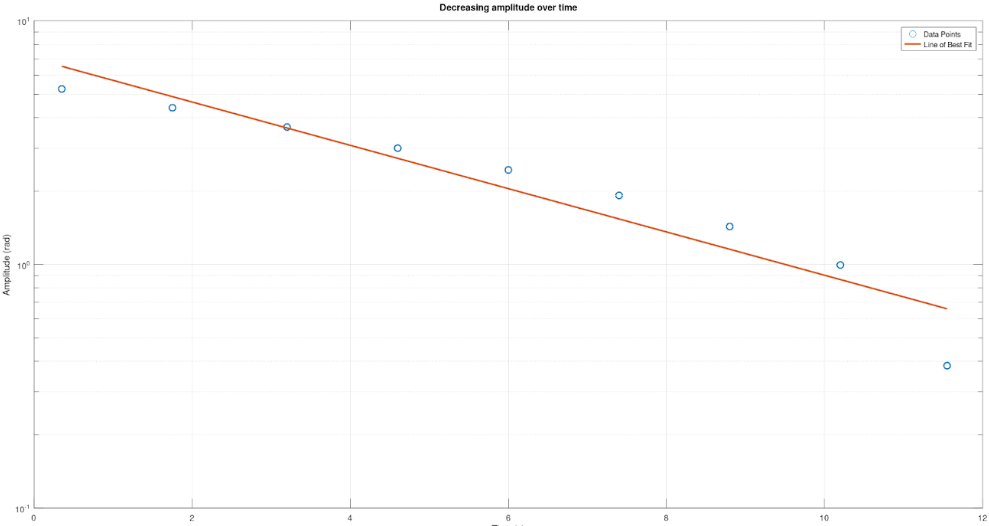
\includegraphics[width=1\textwidth]{oscillations/images/log}
  \caption{Semi-logaritmic plot of the amplitude over time}
  \label{fig:log of damping factor}
\end{figure}

The displacement amplitude $x(t)$ decreases with:
\begin{equation}
  x(t) = e^{-\gamma t} \cos(\omega t + \phi) 
  \label{eq:displacement amplitude}
\end{equation}
The slope of the line of best fit $l$ is equal to the $-\gamma$ term in Equation .
\begin{equation}
  |l| = \gamma 
\end{equation}

By this a damping factor of $\gamma_{direct} = 1.3 \pm 0.2 (rad/s)$ was determined.

\subsection{Indirect Calculation of Damping} \label{sec:indirect_damping}

\begin{figure}[H]
  \centering
  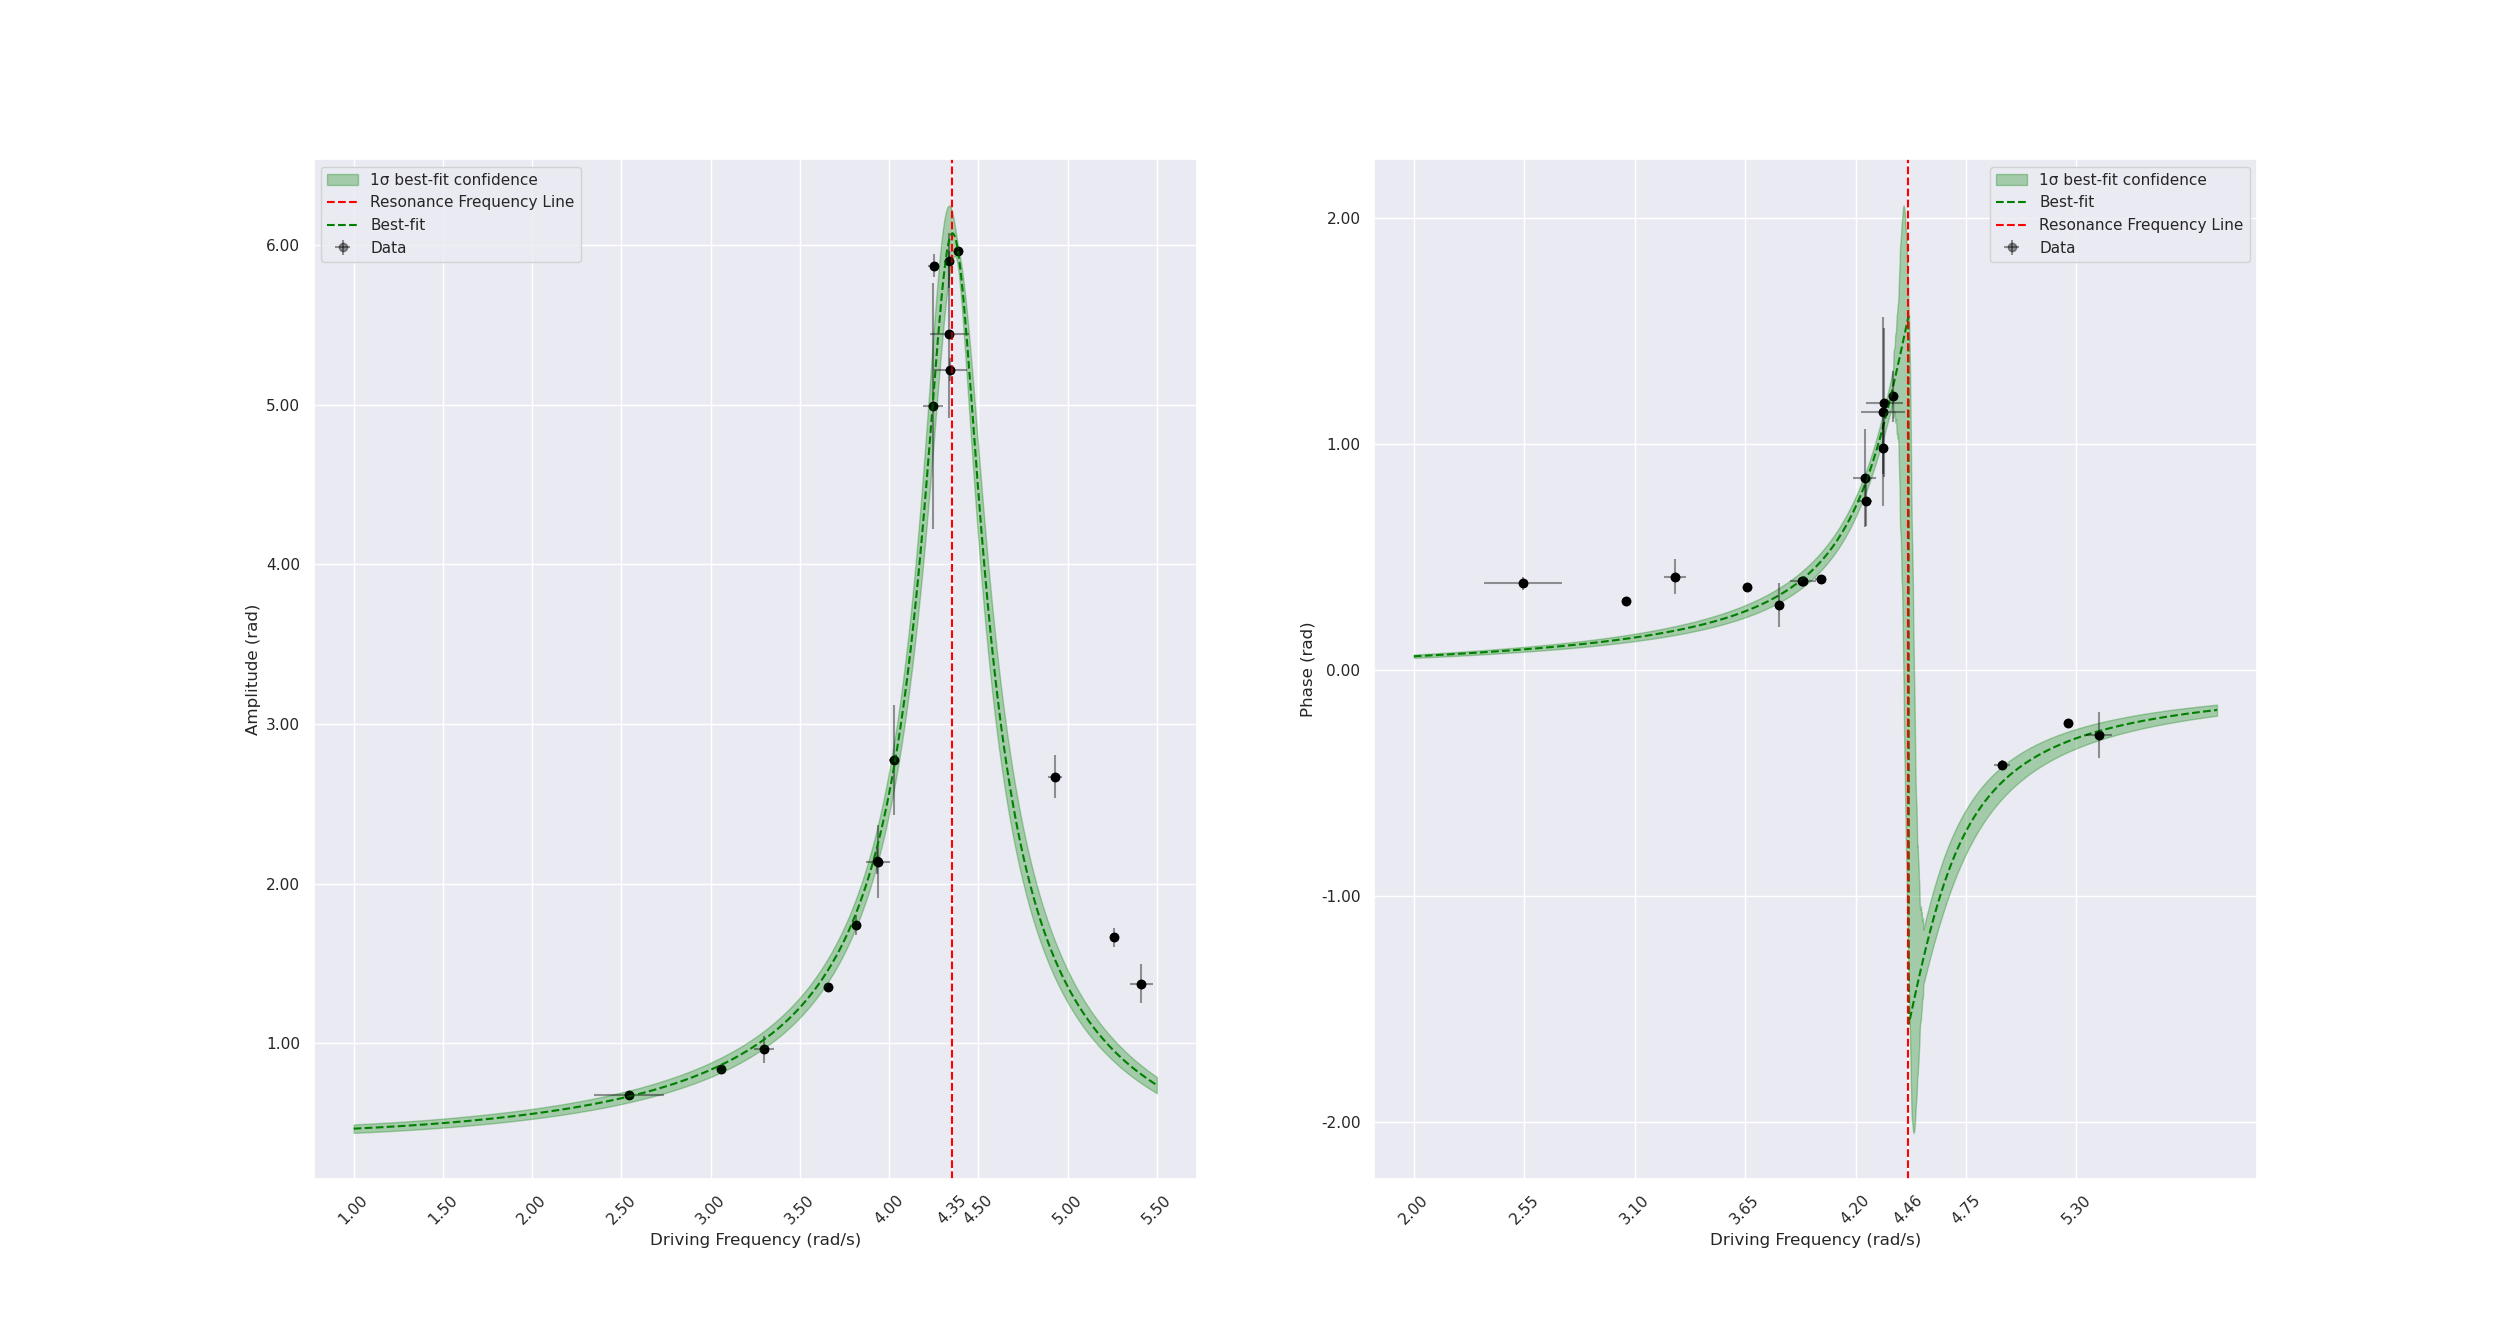
\includegraphics[width=1\textwidth]{oscillations/images/resonance}
  \caption{Amplitude and phase difference of the oscillations plotted against driving frequency.}
  \label{fig:resonance}
\end{figure}

Oscillations of the damped driven system were recorded for different values of the driven force\footnote{There is a linear relation between the driving force and the input voltage.}. The graph of the amplitude and phase difference of the oscillations against driving frequencies with best-fit curves and correspoding uncertanties are depicted in Fig.\ref{fig:resonance}. Tabular data with respective errors are depicted in Table \ref{tab:data}.

Resonance frequency from the amplitude-frequency graph is estimated to be $\omega_{amplitude} = 4.35 \pm 0.09 (rad/s)$. Resonance frequency from the phase-frequency graph is estimated to be $\omega_{phase} = 4.46 \pm 0.02 (rad/s)$. Combined resonance frequency is

\begin{equation*}
\omega_{r} = \frac{\omega_{amplitude} + \omega_{phase}}{2} \pm \sqrt{\sigma(\omega_{amplitude}) + \sigma(\omega_{phase})} = 4.41 \pm 0.09 (rad/s)
\end{equation*}

Damping factor is again evaluated from Eq.~\ref{eq:freq_deps}.

\begin{equation*}
        \gamma_{indirect} = \sqrt{ \frac{\omega^2 - \omega_{res}^2}{2} } = \sqrt{ \frac{4.79^2 - 4.41^2}{2} } = 1.32 \pm 0.8 (rad/s)
\end{equation*}       

This damping factor matches the damping factor previously calculated ($\gamma_{direct}$).

Error analysis for the resonance frequencies and the (indirect) damping factor is located in Appendix \ref{appendix:errors}.

\section{Discussion}

\lipsum{500}

{\color{gray}\hrule}
\begin{center}
\section{Conclusion}
\bigskip
\end{center}
{\color{gray}\hrule}

\begin{multicols}{2}
  \lipsum{1}
\end{multicols}

\appendix
{\color{gray}\hrule}
\begin{center}
\section{Precession Raw Data} \label{sec:appendix:precession_raw_data}
\end{center}
{\color{gray}\hrule}

\begin{multicols}{2}
In figure \ref{fig:appendix:raw_precession_data}, eleven measurements for precession frequency for different torques and initial spinning angular velocities ($\boldsymbol\omega_{3}$) are depicted with their mean values.

Because of the reasons discussed in section TODO, measurements $2, 8$ and $10$ have unique torque-$\boldsymbol\omega_3$ combinations. Thus, they do not have a pair of measurements to calculate the mean squared error for their unique torque-$\boldsymbol\omega_3$ combinations (see appendix \ref{appendix:errors} for error analysis)\footnote{However, their error was estimated by the standard error elicited from their time distribution.}. Consequently, they are referred to as \emph{Type I} measurements in figure \ref{fig:results:processed_precession}.

In contrast, all other measurements have a pair\footnote{That is, these pairs of measurements have the same torque-$\boldsymbol\omega_3$ combination.}, including $\#1 (4/5)$, $\#2 (3/7)$, $\#3 (1/9)$, $\#4 (6/11)$ points. In figure \ref{fig:results:processed_precession}, they are referred to as \emph{Type II} measurements.

\end{multicols}
\begin{figure}[!ht]
  \centering
  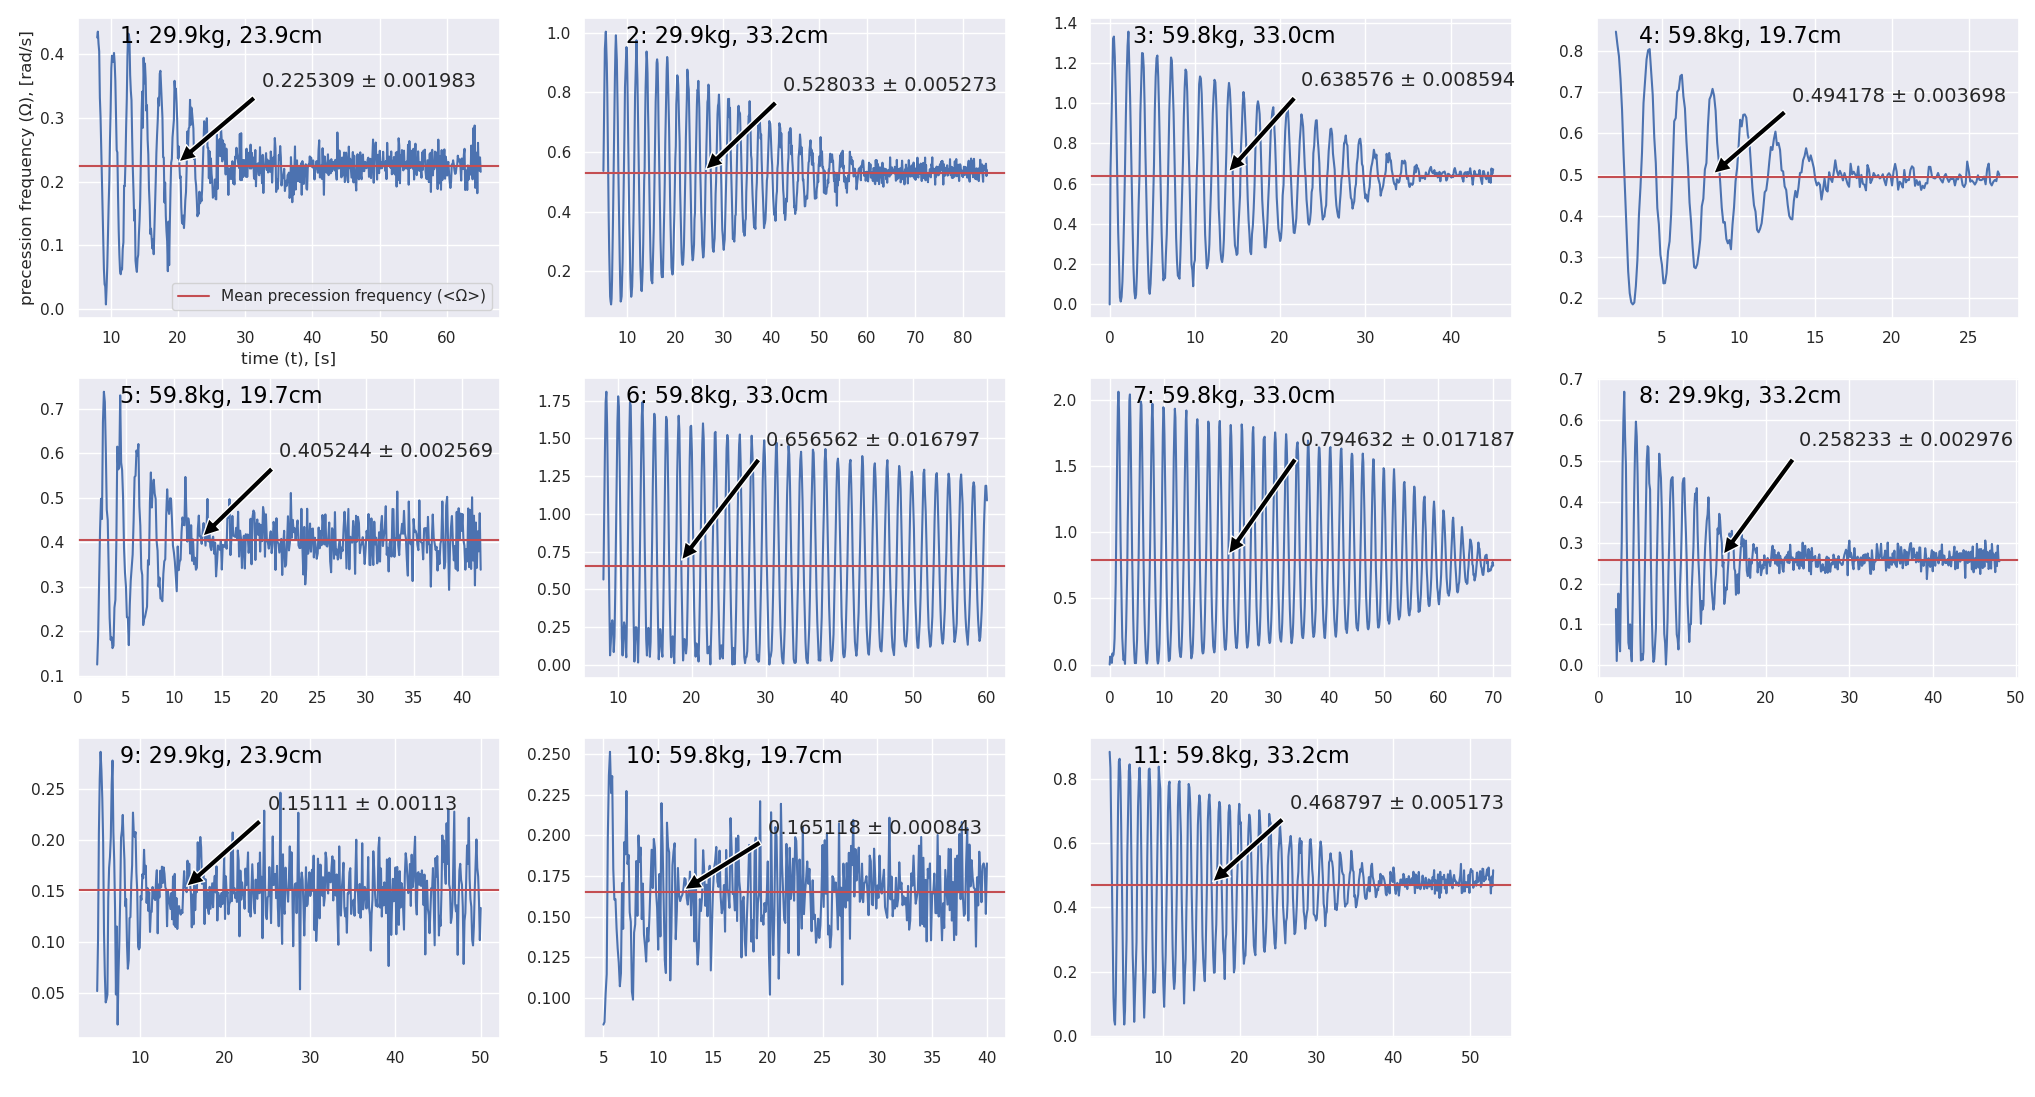
\includegraphics[width=\textwidth]{gyroscope/images/raw_precession}
  \caption{Raw precession frequency data from TISensorTag, and mean values}
  \label{fig:appendix:raw_precession_data}
\end{figure}

\begin{figure}[!ht]
  \centering
  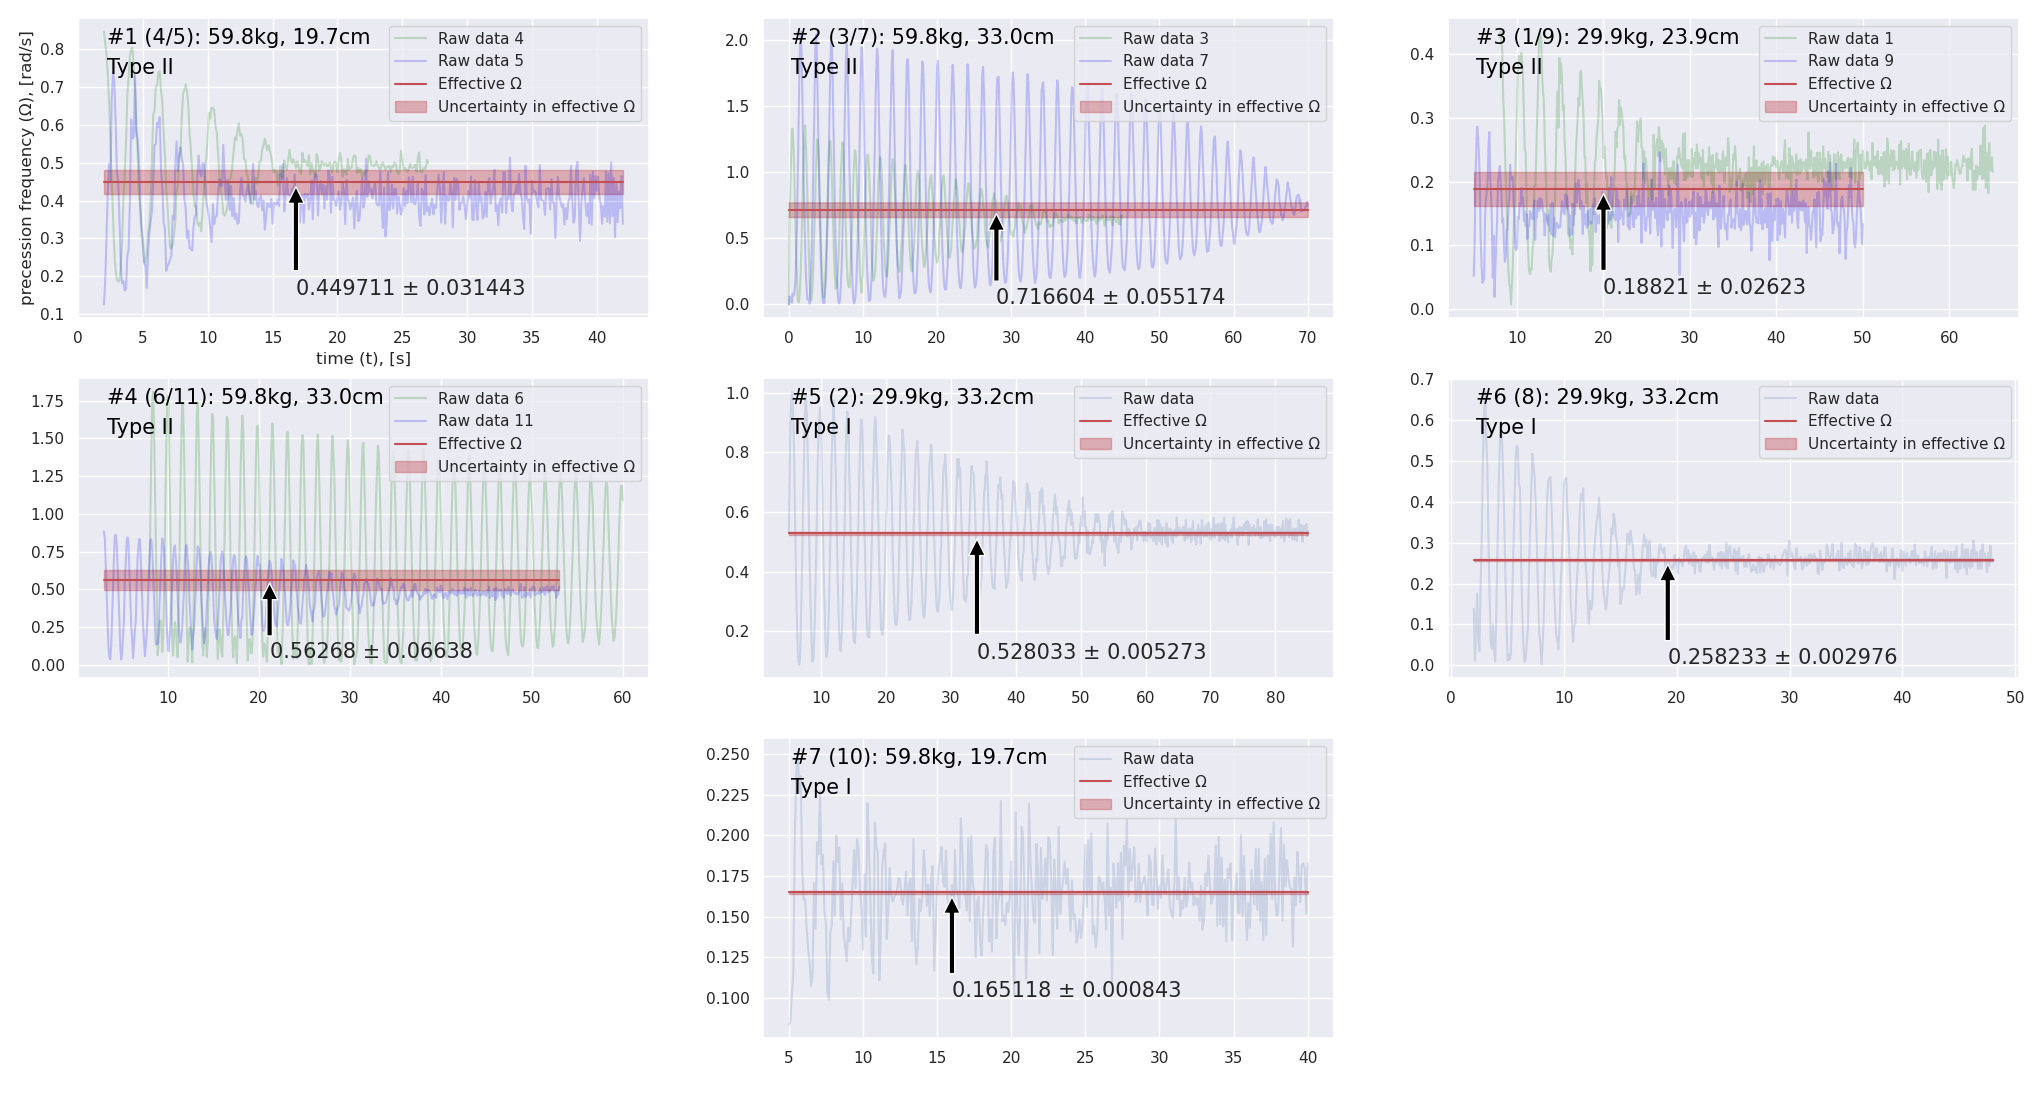
\includegraphics[width=\textwidth]{gyroscope/images/processed_precession}
  \caption{Processed precession frequencies ($\Omega$) }  
  \label{fig:results:processed_precession}
\end{figure}

\begin{multicols}{2}
Table \ref{tab:results:precession} in section \ref{sec:results} contains effective precession frequencies and their uncertainties for each torque-$\boldsymbol\omega_{3}$ combination depicted by the solid red line in figure \ref{fig:results:processed_precession}.
\end{multicols}

\subsection{Natural Frequency from the Amplitudes} \label{appendix:errors:fn_amplitude}

The uncertanty in $T_i$ is given by:
\begin{equation}
  \Delta T = (\frac{timing uncertainty\sqrt(N )})
\end{equation}

The error in the natural frequency gets propagated as:

\begin{equation}
  \Delta f_n = f_n^2\Delta T 
\end{equation}

\subsection{The damping factor from an underdamped oscillator}
In this case, $\Delta \gamma \propto \Delta t_i +\Delta m + \Delta A_i$. Here $\Delta t_i$ is the assigned error of $0.05$s, this being the measurement interfalls. The line of best fit is in the form $y=mx+c$, the uncertainty in the slope is given by:

\begin{equation}
  \Delta m = \sqrt{\frac{\sigma_y^2}{\sum (t_i - \bar{t_i})^2}}
\end{equation}
Where $\sigma_y^2$ denotes the variance in $A_i$, with $\sigma_y^2$ being equal to:

\begin{equation}
\sigma = \sqrt{\sum_{i=1}^{N} {(t_i - \bar{t_i})^2}{f(t_i)}}
\end{equation}

The uncertainty in $A_i$ is calculated by:
\begin{equation}
  s = \sqrt{\frac{1}{N-1}\sum_{i = 1}^{N}(t_i - \bar{t_i})^2}
\end{equation}

Combing the previous stated uncertanties lead to a value of $\Delta \gamma$ that is determined by:
\begin{equation}
  \Delta \gamma = \sqrt{(\Delta m)^2 + \sum_{i=1}^{N} \left[ \left( \frac{\Delta A_i}{t_i} \right)^2 + \left( \gamma \cdot \frac{\Delta t_i}{t_i} \right)^2 \right]}
\end{equation}

\subsection{ Resonance Frequency from the Amplitude Graph } \label{appendix:errors:res_ampl}

In this case, resonance frequency was estimated by finding the peak value of the best-fit curve $A(x, a, b, c) = \frac{a}{\sqrt{(b-x^2)^2 + cx^2}}$. This is done by setting $\frac{\partial A}{\partial x} = 0$. Therefore,

\begin{equation*}
  \frac{\partial}{\partial x} A(x, a, b, c) = \frac{ax(2b-c-2x^2)}{( b^2 + x^2 (-2b + c + x^2) )^{3/2}} = 0 \Rightarrow x = \sqrt{b - c/2}
\end{equation*}

Values for $a$, $b$, and $c$ were obtained using standard statistical optimization techniques that also yielded the covarience matrix for $a$, $b$, and $c$. The values of interest are:
\begin{equation*}
  a = 8.40, b = 19.02, c = 0.10, \Delta b = 0.18, \Delta c = 0.02
\end{equation*}

Therefore, $x = \omega_{amplitude} = \sqrt{19.02 - 0.10 /2} \approx 4.35 (rad/s)$. Error is propagated using:
\begin{equation*}
  \frac{\Delta x}{x} = \sqrt{ \left( \frac{\partial x}{\partial b} \Delta b \right)^2 + \left( \frac{\partial x}{\partial c} \Delta c \right)^2} = \sqrt{ \left( \frac{1}{2\sqrt{b - c/2}} \Delta b \right)^2 + \left( \frac{1}{-4\sqrt{b-c/2}} \Delta c \right)^2} 
\end{equation*}

Plugging the values in, error in the resonance frequency can be computed to be $\Delta x = 0.09 (rad/s)$.

Therefore, $\omega_{amplitude} = 4.41 \pm 0.09 (rad/s)$.

\subsection{ Resonance Frequency from the Phase Graph } \label{appendix:errors:res_phase}

In this case, resonance frequency was estimated by finding the point of discontinuity of the best-fit curve $\phi(x, a, b) = \arctan \frac{ax}{b - x^2}$. For this function, the point of discontinuity coincides with the peak value, so the same statistical optimization techniques were utilized as in section \ref{appendix:errors:res_ampl}. The values and errors of the parameters are:
\begin{equation*}
  a=0.48, b = 19.93, \Delta b = 0.18
\end{equation*}

Resonance frequency is located where $\phi = \pi/2$, thus in the peak-discontinuity point. This equality holds if $b-x^2=0$. Therefore, $x = \sqrt{b} > 0, x = 4.46 (rad/s)$. The error is computed as follows:

\begin{equation*}
  \frac{\Delta x}{x} = \frac{\partial x}{\partial b} \Delta b \Rightarrow \Delta x = \frac{\Delta b}{2\sqrt{b}} = 0.02
\end{equation*}

Therefore, $\omega_{phase} = 4.46 \pm 0.02 (rad/s)$.

\subsection{Damping Factor in terms of Resonance Frequency}

The relation between the damping factor $\gamma$ and natural frequency $\omega$ and the resonance frequency $\omega_{res}$ is
\begin{equation*}
  \gamma = \sqrt{\frac{\omega^2 - \omega_{res}^2}{2}} = 1.32 (rad/s)
\end{equation*}

The error is
\begin{equation*}
  \left( \frac{\Delta \gamma}{\gamma} \right)^2 = \left( \frac{\partial \gamma}{\partial \omega} \Delta \omega \right)^2 + \left( \frac{\partial \gamma}{\partial \omega_{res}} \Delta \omega_{res} \right)^2 = \frac{\omega^2 \Delta \omega}{2(\omega^2 - \omega_{res}^2)} + \frac{\omega_{res}^2\Delta \omega_{res}}{2(\omega^2 - \omega_{res}^2)}
\end{equation*}

\begin{equation*}
  \Delta \gamma = \gamma \sqrt{\frac{\omega^2 \Delta \omega}{2(\omega^2 - \omega_{res}^2)} + \frac{\omega_{res}^2\Delta \omega_{res}}{2(\omega^2 - \omega_{res}^2)}} = \gamma \sqrt{\frac{\omega^2 \Delta \omega + \omega_{res}^2 \Delta \omega_{res}}{2(\omega^2 - \omega_{res}^2)}} 
\end{equation*}
\begin{equation*}
  = 1.32 \sqrt{ \frac{4.78^2 \times 0.02 + 4.41^2 \times 0.09}{2(4.78^2 - 4.41^2)} } = 0.8
\end{equation*}

Therefore,
\begin{equation*}
  \gamma = 1.32 \pm 0.8 (rad/s) 
\end{equation*}


\printbibliography

\end{document}
